\documentclass{article}

\usepackage[utf8]{inputenc}
\usepackage{parskip}
\usepackage[backend=biber]{biblatex}
\usepackage{graphicx}
\usepackage{epstopdf}
\usepackage{wrapfig}
\usepackage{mwe}
\usepackage{libertine}
\usepackage{inconsolata}
\usepackage{hyperref}

\addbibresource{yonac.bib}

\newcommand\theversion{1.0.0-git}

\hypersetup{
  hidelinks,
  pdftitle={Yonac v\theversion},
  pdfauthor={Johann Tutor}
}

\setcounter{secnumdepth}{4}

\begin{document}
\title{Yonac\\ \large A card game, v\theversion}
\author{Johann Tutor}
\date{\today}
\maketitle

Yonac is a quick and easy-to-learn card game developed by Johann Tutor
and Gaetan Boue. Its name is from the Japanese word for ``four'' and
from the first two letters of ``ace''. It is inspired by the game ``Ace
of Spades'', described in Bob Phillips'
\citetitle{ref:supercool}\footfullcite{ref:supercool}.

\tableofcontents

\newpage

\section{Requirements}

Yonac uses a standard deck of cards (jokers optional). Any number of
players may play.

\section{Rules}

The aim of the game is to collect as many cards as possible without
collecting the Ace of Spades.

\subsection{The Cards}
\label{sec:cards}

The four Aces (i.e. the Ace of Spades, the Ace of Hearts, the Ace of Clubs and
the Ace of Diamonds) and Jokers are special and are described below. All other
cards have no special attributes.

A card is described as ``Potent'' if its special attribute may be used.

\subsubsection{The Ace of Spades}
Picking up the Ace of Spades, except when using the Ace of Clubs or the
Ace of Hearts, will result in a loss. The Ace of Spades is always Potent.

\subsubsection{The Ace of Diamonds}
The Ace of Diamonds forces you to add more cards to the Set. The Ace of
Diamonds is Potent on collection and is no longer Potent when it is used
to add more cards to the Set.

\subsubsection{The Ace of Hearts}
The Ace of Hearts allows you to pick up the Ace of Spades once without
losing. The Ace of Hearts becomes Potent after you collect it and your
turn finishes. The usage of this card is described in
\ref{par:spadeshearts}.

\subsubsection{The Ace of Clubs}
The Ace of Clubs gives you one chance to win instantly. The Ace of Clubs
becomes Potent after you collect it and your turn finishes. The usage of
this card is described in \ref{sec:playac}.

\subsubsection{The Joker}
If Jokers are in play, a Joker will remove Aces from a Set, or if there
are no Aces in the Set, you can swap it for another player's Potent
Ace. The usage of this card is described in \ref{par:jokersetaces} and
\ref{par:jokersetnoaces}.

\subsection{Gameplay}
\label{sec:gameplay}

The game proceeds in two phases: the Elimination phase and the Sudden
Death phase. Before starting, agree on the number of players needed to
go into the Sudden Death phase; this is the Threshold. These phases are
further discussed in \ref{sec:elimination} and \ref{sec:sd}.

When the Threshold has been decided, shuffle the deck and spread the
cards out on the table; this is the Pile. Decide on a player order.

On each turn, you may do one of two actions: you may collect cards, or
you may use the Ace of Clubs if you have it set aside.

\subsubsection{Collecting Cards}
\label{sec:collecting}

Each player has a stack of cards, called the Stash, into which collected
cards are put. Any cards put into your Stash lose their Potency and may
not be used again until the card returns to the Pile.

\paragraph{}
\label{par:set}
If you choose to collect cards, pick up one or more cards from the Pile
and display them face-up in front of you. These cards are the Set for
this turn.

\paragraph{}
If the Set does not contain any Aces, put the Set into your Stash.
Your turn is now over and play proceeds to the next player. 

\paragraph{}
If the Set contains the Ace of Spades and you do not have a Potent Ace
of Hearts, you lose and all your cards are reshuffled into the Pile.
Play proceeds to the next player.

\paragraph{}
\label{par:spadeshearts}
If the Set contains the Ace of Spades and you have a Potent Ace of
Hearts, place the Ace of Hearts in your Stash and reshuffle the Set into
the Pile. The Ace of Hearts is now not Potent and it may not be used
again until it returns to the Pile. Note that the Ace of Hearts is not
Potent if it is in the Set with the Ace of Spades; it must have been
collected and set aside in a previous turn for this case to apply. Play
proceeds to the next player.

\paragraph{}
\label{par:jokersetaces}
If the Set contains a Joker and there are Aces in the Set, including an
Impotent Ace of Diamonds if present, remove the Aces and shuffle them into the
Pile. Note that if the Set contains the Ace of Spades, the rules for the Ace of
Spades apply instead. Put the rest of the Set, including any Jokers, into your
Stash. Your turn is now over and play proceeds to the next player.

\paragraph{}
\label{par:jokersetnoaces}
If the Set contains a Joker and there are no Aces in the Set, swap the
Joker with a Potent Ace of another player if one exists.  Remember that
Aces in a player's Stash are not Potent. To perform the swap, place the
Joker into the other player's Stash. Take the Potent Ace and put it into
your Set. Do this for every Joker in your Set. If there are no Potent
Aces, then you many not perform a swap. After this, the Jokers lose
their Potency. Continue to evaluate the Set, including any swapped Aces.

\paragraph{}
If the Set contains a Potent Ace of Diamonds, pick up one or more cards
from the Pile and add them to the Set. Re-evaluate the new Set, with the
Ace of Diamonds now no longer Potent.

\paragraph{}
If the Set contains the Ace of Clubs, put the Ace of Clubs aside; the
Ace of Clubs is now Potent. You may play it in a later turn as described
in \ref{sec:playac}.

\paragraph{}
If the Set contains the Ace of Hearts, put the Ace of Hearts aside; the
Ace of Hearts is now Potent. It will protect you if you collect the Ace
of Spades in a later turn as previously described in
\ref{par:spadeshearts}.

Put the remaining cards in the Set into your Stash. Your turn is now
over and play proceeds to the next player.

\subsubsection{Playing the Ace of Clubs}
\label{sec:playac}

If you have a Potent Ace of Clubs, you may choose to play it instead of
collecting cards. Once played and put in your Stash, the Ace of Clubs
loses its Potency and may not be used again until it is returned to the
Pile.

\paragraph{}
To play the Ace of Clubs, declare that you will be playing the Ace of
Clubs. Put the Ace of Clubs in your Stash, then pick up one card from
the Pile and display it face-up in front of you.

\paragraph{}
If the card is not an Ace, put it in your Stash. Your turn is now over
and play proceeds to the next player.

\paragraph{}
If the card is the Ace of Spades, play stops and you win the game.

\paragraph{}
If the card is a Joker, swap it for another player's Potent Ace as
described in \ref{par:jokersetnoaces}. If no player has a Potent Ace,
you may not perform the swap. Evaluate the new card as if that was the
card you picked up.

\paragraph{}
If the card is the Ace of Hearts, put it aside; the Ace of Hearts is now
Potent. Your turn is over and play proceeds to the next player.

\paragraph{}
If the card is the Ace of Diamonds, put it in your Stash and pick up one
more card from the Pile. Re-evaluate the new card.

% If the card is the Ace of Clubs, you're doing it wrong.

\subsubsection{Phase 1: Elimination}
\label{sec:elimination}

During the Elimination phase, players who pick up the Ace of Spades and
lose are eliminated. Play continues until the number of players left
reaches the Threshold, at which point the Elimination phase is over and
the Sudden Death phase begins.

\subsubsection{Phase 2: Sudden Death}
\label{sec:sd}

In the Sudden Death phase, if a player picks up the Ace of Spades and
loses, the game ends. The remaining players will count the number of
cards in their Stash, including any Aces set aside.

\subsubsection{Winning}

There are two ways to win: by picking up the Ace of Spades while using
the Ace of Clubs as described in \ref{sec:playac}, or by not being
eliminated and having the most cards your Stash at the end of the Sudden
Death phase.

In the event of a tie, the tied player who has the Ace of Hearts wins.
If no one has the Ace of Hearts, the tied player with the Ace of Clubs
wins. If no one has the Ace of Hearts or the Ace of Clubs, the tied
player with the Ace of Diamonds wins. If no one has any Aces, the tied
player who had a turn last wins. Note that these Aces do not need to be
Potent to count. Also note that if none of the remaining players have
had a turn, then the player last in the queue wins.

\section{Glossary}
\begin{description}
  \item[Elimination Phase](\ref{sec:elimination})\\
    The first phase. In this phase, the game does not end when a loss
    occurs.
  \item[Pile](\ref{sec:gameplay})\\
    The uncollected cards spread out. In each turn, all cards are taken
    from the Pile.
  \item[Potent](\ref{sec:cards})\\
    Describes a card whose special attribute may be used.
  \item[Set](\ref{par:set})\\
    The cards picked up during a turn.
  \item[Stash](\ref{sec:collecting})\\
    The player's collected cards. Each player's Stash is
    counted at the end of the game. Used Aces are put in the Stash and
    may not be played again until the Ace is returned to the Pile.
  \item[Sudden Death Phase](\ref{sec:sd})\\
    The second phase. In this phase, the game ends when a loss occurs.
  \item[Threshold](\ref{sec:gameplay})\\
    The number of players needed to go into the Sudden
    Death phase.
\end{description}

\newpage
\section{Credits}

This game was inspired by Bob Phillips' ``Ace of Spades''.

The game was suggested by Johann Tutor on July 28, 2016.

The special attributes for the Ace of Hearts and the Ace of Clubs were
suggested by Gaetan Boue. The special attribute for the Ace of Diamonds
was suggested by Onie Tam.

The rules were refined and formalized by Johann Tutor and Gaetan Boue.

This document was written by Johann Tutor.

\medskip
\hrule

{
  \small
  \includegraphics[scale=0.5]{cc-by.eps}\\
  This work is licensed under the Creative Commons Attribution 4.0
  International License. To view a copy of this license, visit
  \url{http://creativecommons.org/licenses/by/4.0/} or send a letter to Creative Commons, PO Box 1866, Mountain View, CA 94042, USA.
}

\end{document}
